% Define document class
\documentclass[modern]{aastex631}

% Filler text
\usepackage{blindtext}

% Commands
\newcommand{\dd}{\mathrm{d}}
\newcommand{\diff}[2]{\frac{\dd #1}{\dd #2}}
\newcommand{\mean}[1]{\left\langle #1 \right\rangle}
\newcommand{\chieff}{\chi_{\mathrm{eff}}}

% Begin!
\begin{document}

% Title
\title{Gar\c{c}on: Spins Please (Or Some Other Pun-y Title)}

% Institutional Addresses
\newcommand{\cca}{Center for Computational Astrophysics, Flatiron Institute, New York NY 10010, USA}
\newcommand{\sbu}{Department of Physics and Astronomy, Stony Brook University, Stony Brook NY 11794, USA}

% Author list
\author[0000-0003-1540-8562]{Will M. Farr}
\email{will.farr@stonybrook.edu}
\affiliation{\sbu}
\affiliation{\cca}

\author{Maya Fishbach}

\author{Thomas Callister}

\author{Vicky Kalogera}

\author{Katie Breivik}

\author{Daniel Holz}

\author{Simona Miller}

\author{Sharan Banagiri}

\author{and friends}

% Abstract with filler text
\begin{abstract}
We show various models for the distribution of black hole spin vectors in
GWTC-3 and discuss what they might imply about the evolution of these systems.
\end{abstract}

% Main body with filler text
\section{Introduction}

Blah.

\section{Building Intuition}

\begin{figure}
    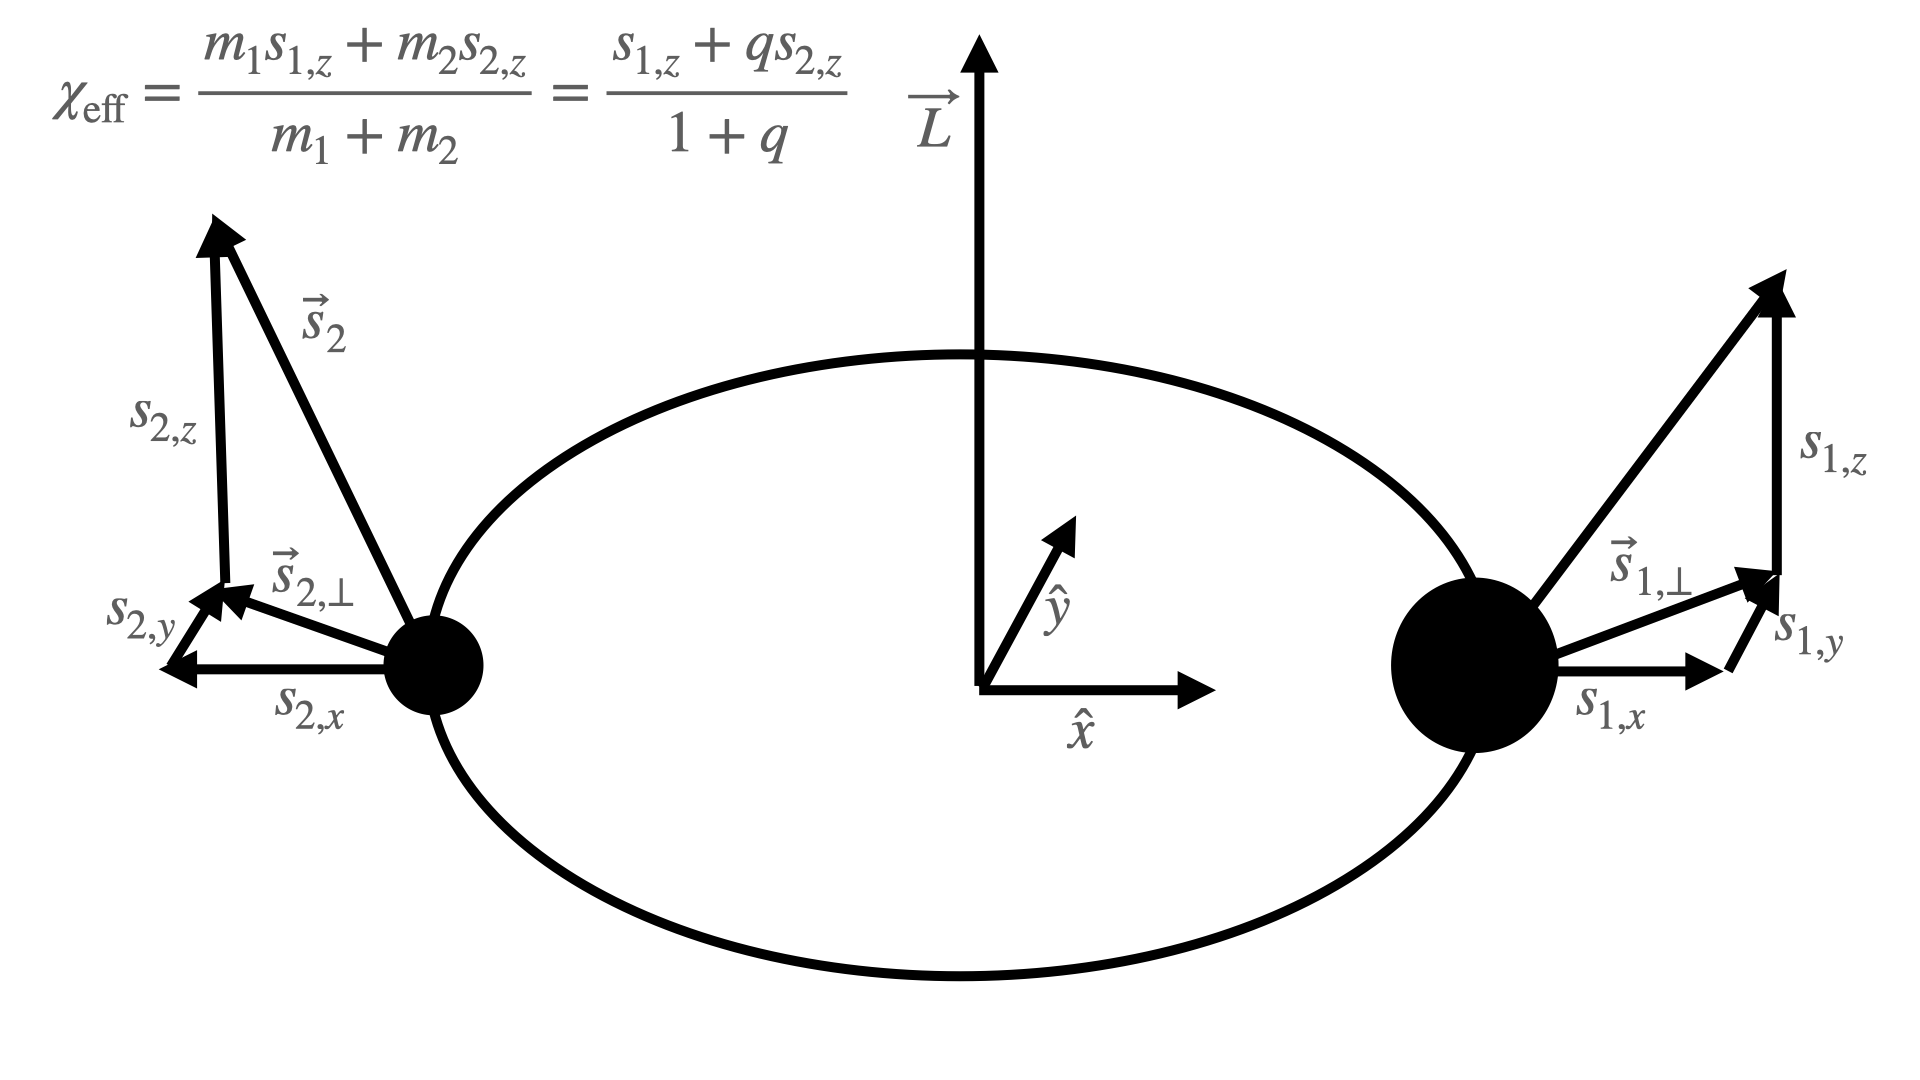
\includegraphics[width=\columnwidth]{static/SpinFigure.png}
    \caption{\label{fig:SpinFigure} A figure showing the coordinate system we
    use for spins.}
\end{figure}

[This argument was originally suggested by Maya, and fleshed out by Vicky and
Will at Aspen.]  Note that 
\begin{equation}
    \chieff = \frac{s_{1,z} + q s_{2,z}}{1+q}
\end{equation}
where $s_{i,z}$ is the $z$-component (the out-of-orbital-plane component) of the
spin of the $i$ object and $q = m_2 / m_1 < 1$.  If we assume that the
distribution of the $\vec{s}_i$ in the population do not depend on $q$, then by
linearity of expectation values, we have 
\begin{equation}
    \mean{\chieff} = \frac{\mean{s_{1,z}} + q \mean{s_{2,z}}}{1+q}
\end{equation}
and 
\begin{equation}
    \diff{\mean{\chieff}}{q} = \frac{\mean{s_{2,z}} - \mean{s_{1,z}}}{\left( 1 + q \right)^2}.
\end{equation}
\citet{Callister2021} showed that the GWTC-2 \citep{Abbott2021GWTC-2} population
of binary black hole mergers have 
\begin{equation}
    \mean{\chieff}\left( q = 0.8 \right) \simeq 0.04
\end{equation}
and
\begin{equation}
    \diff{\mean{\chieff}}{q} \simeq -0.46
\end{equation}
(we have chosen to evaluate the \citet{Callister2021} mean $\chieff$ at the
best-constrained mass ratio of $q \simeq 0.8$).  The GWTC-3 catalog exhibits the
same correlations, with reduced uncertainty \citep{Abbott2021GWTC-3}.  These
properties of the population imply 
\begin{eqnarray}
    \mean{s_{1,z}} & \simeq & 0.70 \\
    \mean{s_{2,z}} & \simeq & -0.79.
\end{eqnarray}
Even accounting for the uncertainties in \citet{Callister2021}'s population,
that the mean $\chieff$ is close to zero at nearly-equal masses imples that
$\mean{s_{1,z}} \simeq - \mean{s_{2,z}}$.  That $\chieff$ decreases with
increasing $q$ implies that $\mean{s_{2,z}} < \mean{s_{1,z}}$, so that
$\mean{s_{2,z}}$ must be negative while $\mean{s_{1,z}}$ is positive
\emph{assuming that the spin distribution is independent of the system mass
ratio $q$}.


\bibliography{bib}

\end{document}
